\documentclass[12pt]{article}
\usepackage[margin=1in]{geometry} 
\usepackage[shortlabels]{enumitem}
\usepackage{caption}
\usepackage{algorithm}
\usepackage[noend]{algpseudocode}
\usepackage[table,xcdraw]{xcolor}
\usepackage{import}
\usepackage{tikz}
\usepackage{tikz,fullpage}
\usetikzlibrary{arrows,%
                petri,%
                topaths}%
\usepackage{tkz-berge}
\usepackage[position=top]{subfig}
\usepackage{amsmath,amsthm,amssymb,amsfonts, enumitem, fancyhdr, color, comment, graphicx, environ}
\pagestyle{fancy}
\setlength{\headheight}{65pt}
\newenvironment{problem}[2][Problem]{\begin{trivlist}
\item[\hskip \labelsep {\bfseries #1}\hskip \labelsep {\bfseries #2.}]}{\end{trivlist}}
\newenvironment{sol}
    {\emph{Solution:}
    }
    {
    \qed
    }
\specialcomment{com}{ \color{blue} \textbf{Comment:} }{\color{black}} %for instructor comments while grading
\NewEnviron{probscore}{\marginpar{ \color{blue} \tiny Problem Score: \BODY \color{black} }}
% creates keywords for input and output in algorithm block
\algblock{Input}{EndInput}
\algnotext{EndInput}
\algblock{Output}{EndOutput}
\algnotext{EndOutput}
\newcommand{\Desc}[2]{\State \makebox[13em][l]{#1}#2}
\lhead{Mazen Alotaibi \textit{(alotaima)}}
\rhead{CS 420 \\ Section 001 \\ Winter 2019 \\ HW 3}

\begin{document}

\begin{problem}{1} A region contains a number of towns connected by roads...
\begin{enumerate}[(a)]
    \item What algorithm would you recommend be used to find the fastest route ...
    \item  Suppose one ”optimal” location (maybe instead of G) must be selected for the fire station such that it minimizes the distance ...
    \item  Now suppose you can build two fire stations.  Where would you ...
\end{enumerate}
\end{problem}
\begin{sol}
\begin{enumerate}[(a)]
    \item Using Dijkstra's algorithm will find the shortest path from G. Refer to Table 1 for an example run. It will take $O(r+f\ log(f))$ to run the Dijkstra's algorithm using Fibonacci heap.

    \item  Applying Dijkstra's algorithm for each vertex as a separate source and use Fibonacci heap as the data structure. In every run, get the maximum extractMin from every Fibonacci heap of every run, then pull the lowest maximum extractMin from all runs to get the optimal source vertex. It will take $O(f)$ to loop through all vertices as source and $O(r+f\ log(f))$ to run the Dijkstra's algorithm using Fibonacci heap, so the total run time is $O(rf+f^2\  log(f))$. The optimal location to place a fire statios for this graph is C.
    \item  They are multiple ways to answer this question:
    \begin{enumerate}
        \item Simple: Using Dijkstra's algorithm, loop through all possible way to select two fire stations, then pick the two disjoints that has the lowest some of two paths with lowest overlaps of those paths. It will take $O(f^2)$ to loop through all vertices to select two sources and $O(r+f\ log(f))$ to run the Dijkstra's algorithm using Fibonacci heap, so the total run time is $O(rf^2+f^3\  log(f))$. The optimal locations to place two fire stations for this graph are C and G.
        \item Advanced: Using Suurballe's algorithm, the algorithm finds two disjoint paths in a non-negativelyweighted directed graph with the lowest sum, so at the end the pair would connect at the end. Although this example is undirected graph, can assume that a path of undirected edge of X and Y of weight W has two directed edges from X to Y and Y to X with W weight for each edge. Therefore, it will take $O(r+f\ log(f))$ to run the algorithm.
    \end{enumerate}
    
\end{enumerate}
\end{sol}

\begin{problem}{2} Consider an undirected graph G=(V,E) with nonnegative edge weights...
\end{problem}
\begin{sol}
After updating all weights of a graph by adding one, the shortest path may change. I have created a simple graph, \textit{Graph 1}, as an example. Let assume that the source position is $s$ and the final position is $f$. Before updating the graph, the shortest path was $s->b->d->f$, which has a path cost of 4 units. After updating the graph, \textit{Graph 2}, the shortest path was $s->a->f$, which has a path cost of 7, which is less than $s->b->d->f$ which has a oath cost of 8. Proving by contradiction, when updating the weights of edges, the shortest path may change.
\end{sol}

\begin{problem}{3} Does the shortest path between two vertices on a...
\end{problem}
\begin{sol}
No. For example, in the graph, \textit{Graph 3}, the shortest path from $s$ to $f$ is $s->f$, which has the weight of 4 units. However, the minimal spanning tree will have $s->a->f$, which has a total weight of 6 units. Hence, the shortest path between two vertices doesn't always lie in the minimal spanning tree.

\end{sol}
\newpage

\begin{table}[]
    \begin{center}
    \begin{tabular}{|l|l|l|}
        \hline
        \rowcolor[HTML]{C0C0C0} 
        \textbf{V} & \textbf{D} & \textbf{shortest path} \\ \hline
        G          & 0          & G                      \\ \hline
        A          & 12         & G-E-D-C-A              \\ \hline
        B          & 6          & G-H-B                  \\ \hline
        C          & 8          & G-E-D-C                \\ \hline
        D          & 5          & G-E-D                  \\ \hline
        E          & 2          & G-E                    \\ \hline
        F          & 8          & G-H                    \\ \hline
        H          & 3          & G-H                    \\ \hline
    \end{tabular}
    \caption*{Table 1: An Example Run for Problem 1.a)}
    \end{center}
\end{table}
\begin{figure}[h]
\begin {center}
\begin{tikzpicture}[auto, node distance=3cm, every loop/.style={},
                    thick,main node/.style={draw,font=\sffamily\Large\bfseries}]

  \node[main node] (1) {a};
  \node[main node] (2) [below of=1] {s};
  \node[main node] (3) [right of=2] {b};
  \node[main node] (4) [right of=3] {c};
  \node[main node] (5) [right of=4] {d};
  \node[main node] (6) [right of=5] {f};

  \path[every node/.style={font=\sffamily\small}]
    (1) edge node [left] {3} (6)
        edge node [right] {2} (2)
    (2) edge node [right] {1} (3)
    (3) edge node [right] {1} (4)
    (4) edge node [right] {1} (5)
    (5) edge node [right] {1} (6);
\end{tikzpicture}
\caption*{Graph 1: Before Updating the Graph for Problem 2}
\end{center}
\centering
\end{figure}

\begin{figure}[h]
\begin {center}
\begin{tikzpicture}[auto, node distance=3cm, every loop/.style={},
                    thick,main node/.style={draw,font=\sffamily\Large\bfseries}]

  \node[main node] (1) {a};
  \node[main node] (2) [below of=1] {s};
  \node[main node] (3) [right of=2] {b};
  \node[main node] (4) [right of=3] {c};
  \node[main node] (5) [right of=4] {d};
  \node[main node] (6) [right of=5] {f};

  \path[every node/.style={font=\sffamily\small}]
    (1) edge node [left] {4} (6)
        edge node [right] {3} (2)
    (2) edge node [right] {2} (3)
    (3) edge node [right] {2} (4)
    (4) edge node [right] {2} (5)
    (5) edge node [right] {2} (6);
\end{tikzpicture}
\caption*{Graph 2: After Updating the Graph for Problem 2}
\end{center}
\centering
\end{figure}

\begin{figure}[h]
\begin {center}
\begin{tikzpicture}[auto, node distance=3cm, every loop/.style={},
                    thick,main node/.style={draw,font=\sffamily\Large\bfseries}]

  \node[main node] (1) {a};
  \node[main node] (2) [right of=1] {s};
  \node[main node] (3) [below of=1] {f};

  \path[every node/.style={font=\sffamily\small}]
    (1) edge node [left] {1} (2)
        edge node [right] {5} (3)
    (2) edge node [right] {4} (3);
\end{tikzpicture}
\caption*{Graph 3: Example Graph for Problem 3}
\end{center}
\centering
\end{figure}

\end{document}
